\documentclass{beamer}
\setbeamercovered{transparent}

\usepackage{epstopdf}
\usepackage[inline]{asymptote}

\mode<presentation> %?

\usetheme{Frankfurt}
\usepackage{helvet}
\usepackage{mathptmx}
%\usefonttheme{professionalfonts}
\usefonttheme[onlymath]{serif}
\usefonttheme{structurebold}

%\renewcommand{\familydefault}{Futura}
%\setsansfont{Verdana}

\setlength{\unitlength}{\paperwidth}

% width, height, title, content
\newcommand{\SizedBlock}[4]{
  \begin{block}{#3}
    \parbox[t][#2\paperwidth][t]{#1\paperwidth}{#4}    
  \end{block}
}

% w1, c1, w2, c2
\newcommand{\TwoColumns}[4]{
  \vspace{-0.02\paperwidth}
  \begin{columns}[t]
    \begin{column}{#1\paperwidth}
      #2
    \end{column}\hspace{-0.02\paperwidth}
    \begin{column}{#3\paperwidth}
      #4
    \end{column}
  \end{columns}
}

% w1, c1, w2, c2, w3, c3
\newcommand{\ThreeColumns}[6]{
  \vspace{-0.02\paperwidth}
  \begin{columns}[t]
    \begin{column}{#1\paperwidth}
      #2
    \end{column}\hspace{-0.07\paperwidth}
    \begin{column}{#3\paperwidth}
      #4
    \end{column}\hspace{-0.07\paperwidth}
	\begin{column}{#5\paperwidth}
      #6
    \end{column}
  \end{columns}
}

% height, title1, content1, title2, content2
\newcommand{\TwoColumnBlocksW}[6]{
  \TwoColumns{
        #6}{
        \SizedBlock{#6}{#1}{#2}{#3}}{
        #6}{
        \SizedBlock{#6}{#1}{#4}{#5}}
}

% height, title1, content1, title2, content2
\newcommand{\TwoColumnBlocks}[5]{
  \TwoColumnBlocksW{#1}{#2}{#3}{#4}{#5}{0.4}
}

% height, title1, content1, title2, content2, title3, content3
\newcommand{\ThreeColumnBlocks}[7]{
  \ThreeColumns{
        0.24}{
        \SizedBlock{0.24}{#1}{#2}{#3}}{
        0.24}{
        \SizedBlock{0.24}{#1}{#4}{#5}}{
        0.24}{
        \SizedBlock{0.24}{#1}{#6}{#7}}
}

\newcommand{\PutPic}[3]{
  \put(#1){\includegraphics[#2\paperwidth]{./img/#3}}
}

\usepackage{color}
\usepackage{fancybox}

\begin{document}
\title{Integer-Grid Maps for Quad Meshing\\
\small{[David Bommes et.al Sig 2013]}}
\author{Tengfei Jiang}

\newcommand{\FPP}[2]{\frac{\partial #1}{\partial #2}}
\begin{frame}
  \titlepage
\end{frame}

\begin{frame}{Pipeline}
  \begin{enumerate}
    \item Motivation 
    \item Key Idea
    \item Algorithm
    \item Results
    \item Conclusion
  \end{enumerate}
\end{frame}

\section{Motivation}
\begin{frame}{Motivation \& Related Work}
\begin{block}{Key Problems inside Quad Meshing}
\begin{itemize}
\item Singularity location. Three branches:
  \begin{itemize}
    \item \textcolor{blue}{Frame Field Design}: orthogonal(``Mixed,Global Optimal...'')/in-orthogonal(``Conjugate Direction Field'')
    \item \textcolor{blue}{Metric Design to redistribute Gaussian Curvature}: cone singularity (``incremental flattening'').
    \item \textcolor{blue}{Coarse Quad layer}: Spectral method (``Dong 2006'',''Huang 2008'')
  \end{itemize}
\item Locally injective parameterization: \\local stiffening(``Mixed'')/anti-flip (``Bounded Distortion'')
\item MIQP Solver: greed rounding (``Mixed'')
\item Size/Direction Control: (``Huang 2008'' ``A wave based'')
\end{itemize}
\end{block}
\end{frame}

\begin{frame}{Background}
\begin{eqnarray}
\min &\quad E(f(x))=\frac{1}{2}\sum_{t\in T}A_t\|\nabla f_t - R_tH_t\|^2\\
s.t. &g_{i\to j}(x) = R_{90}^{r_{ij}}(x)+t_{ij} \\
& f^{-1}(s_i) \in Z^2, \forall s_i\in S\\
&det[v-u,w-u] > 0
\end{eqnarray}
\end{frame}

\section{Key Idea}
\begin{frame}{Key Idea}
Simplify the former problem with a known cross-field, thus eqn 2 is a linear constraint. The unknown things
are : 1.$det[v-u,w-u]>0$,  2. $f^{-1}(s_i)$.
\begin{itemize}
\item For eqn (4), define a stronger convex subset.
\item For eqn (3), use improved branch-and-cut solver.
\end{itemize}
\end{frame}

\section{Algorithm}
\begin{frame}{Whole pipeline}
\begin{figure}
\centering
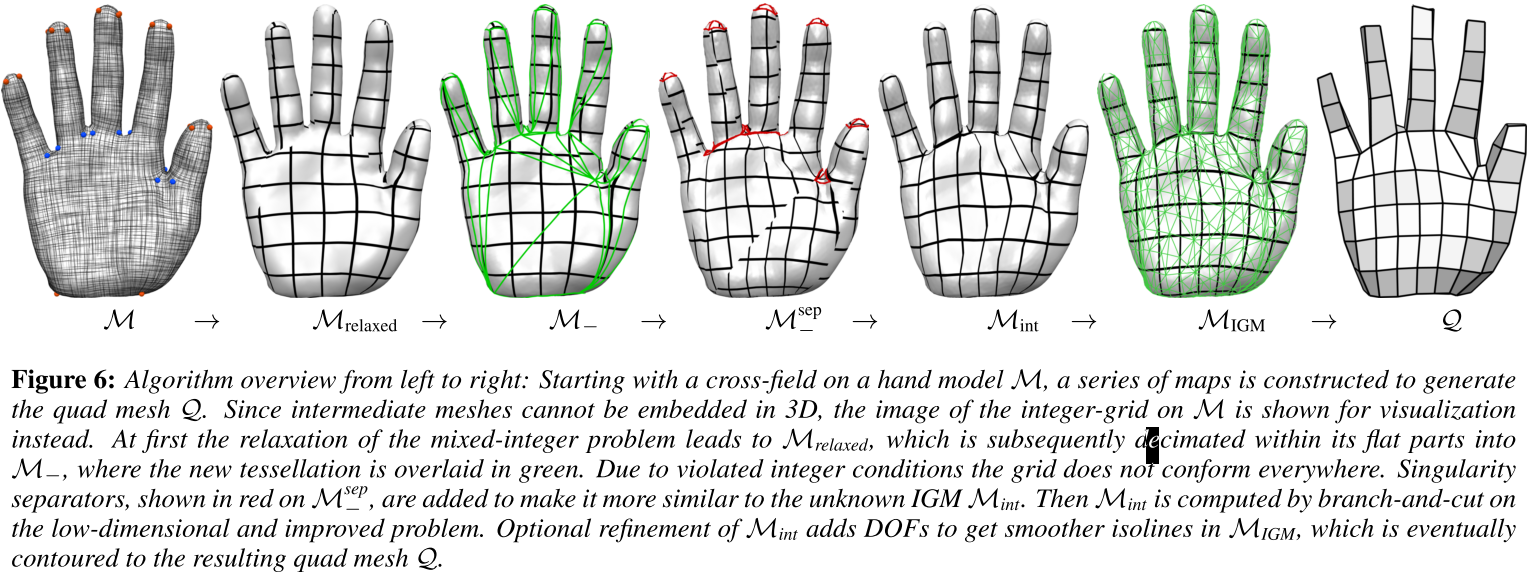
\includegraphics[height=1.7in]{./img/pipeline.png}
\end{figure}
\end{frame}


\begin{frame}{Anti-flip}
\begin{block}{Anti-flip condition}
\begin{eqnarray}
S_i=\{u\in R^2: (u-m)\cdot s_i^{\perp}>0 \land (u-m)\cdot s_{i+1}^{\perp}<0\}
\end{eqnarray}
\end{block}
\begin{figure}[!htb]
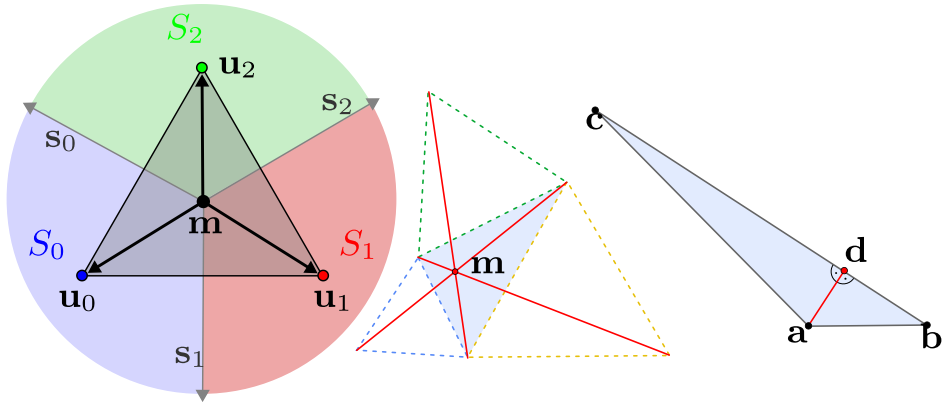
\includegraphics[height=1.5in]{./img/anti-flip.png}
\end{figure}
\end{frame}

\begin{frame}{branch-and-cut solver}
\begin{block}{A simple case}
\begin{eqnarray}
\min &z := −6x_1-5x_2\\
s.t\quad &3x_1+x_2\leq 11 \\
&-x_1+2x_2\leq 5 \\
&x_1,x_2 \geq 0, integer
\end{eqnarray}
\end{block}
\end{frame}

\begin{frame}{A simple case}
\TwoColumns{0.4}{
\begin{figure}[!htb]
\centering
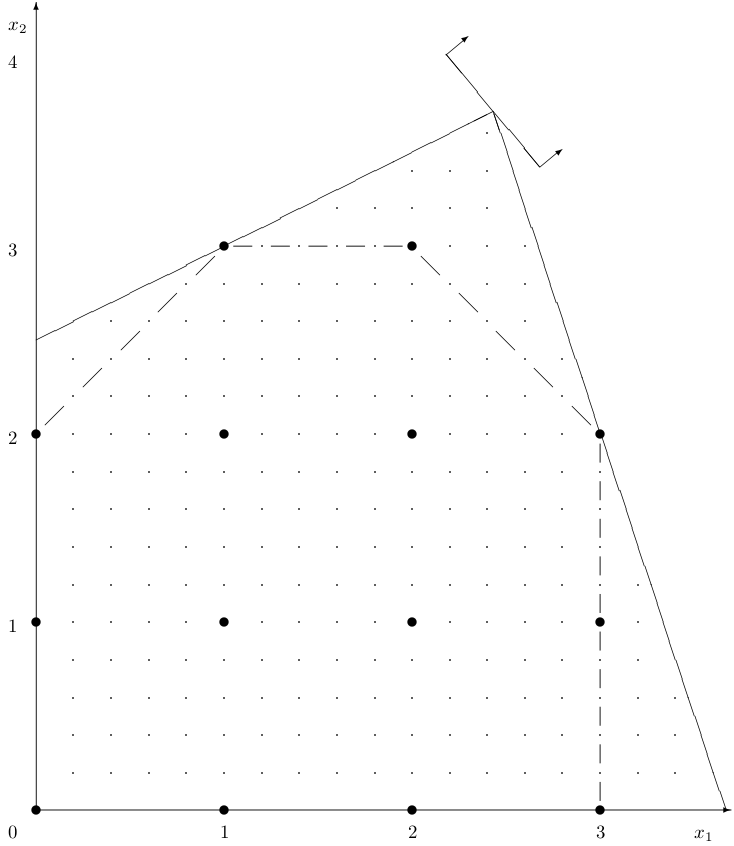
\includegraphics[height=2in]{./img/simple-case-0.png}
\end{figure}
}{0.5}{
\begin{figure}[!htb]
\centering
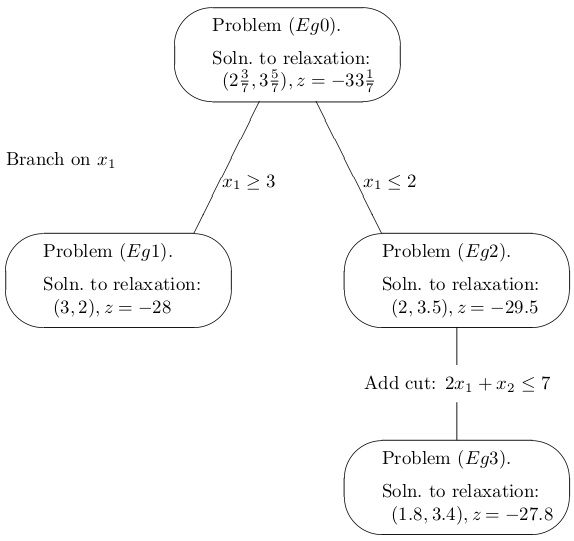
\includegraphics[height=2in]{./img/simple-case-1.png}
\end{figure}
}
\end{frame}

\begin{frame}{Improved Branch-and-cut solver}
\begin{itemize}
\item Complex Reduction: Mesh Decimation
  
\item Singularity Separation
\end{itemize}
\end{frame}


\begin{frame}{Mesh Decimation}
\begin{block}{Basic operations}
\TwoColumns{0.4}{
\begin{figure}
\centering
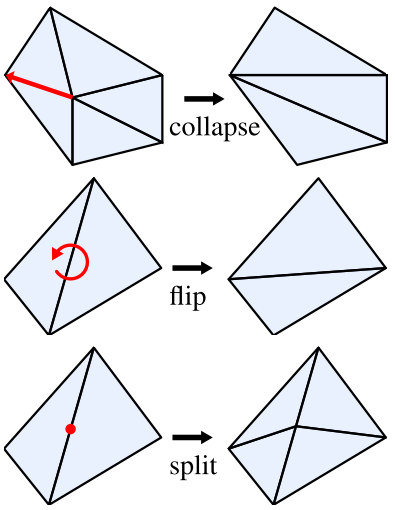
\includegraphics[height=1.5in]{./img/remesh-operation.png}
\end{figure}
}{0.5}{
\begin{figure}
\centering
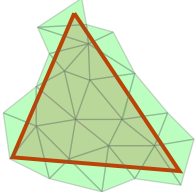
\includegraphics[height=1.5in]{./img/remesh-aim.png}
\end{figure}
}
\end{block}
\begin{itemize}
%\item Q1: How to maintain the mapping function $f:M_{-}\to M$?
\item Q2: How to measure the distortion between $M_{int}$ and $M$ based on $M_{-}$?
\end{itemize}
\end{frame}

%\begin{frame}{Maintain Transition}
%\end{frame}

\begin{frame}{Distortion Measurement}
\begin{block}{}
\TwoColumns{0.3}{
\begin{eqnarray*}
E(f) = \frac{1}{2}\sum_{t\in T}A_t\|R_t^T\nabla f_t - H_t\|^2
\end{eqnarray*}
}{0.4}{
\begin{eqnarray*}
f_{M_{int}\to M}: \underbrace{f_{M_{-}\to M}}_f \circ \underbrace{f_{M_{int}\to M_{-}} }_g
\end{eqnarray*}
}
\begin{block}{}
\begin{eqnarray}
E(f\circ g) = \frac{1}{2}\sum\sum_{t\in T_M,s\in T_{M_{-}}} A_{t\cap f(s)}\|R^T_t\nabla f_t \nabla g_s - H_t\|^2\\
R_t^T\nabla f_t\approx H_t\\
E(f\circ g) \approx \frac{1}{2}\sum{s\in T_{M_{-}}} A_{s}\|\nabla g_s - I\|^2
\end{eqnarray}
\end{block}
\end{block}
\end{frame}

\begin{frame}{Singularity Separation}
\TwoColumns{0.3}{
\begin{figure}[!htb]
\centering
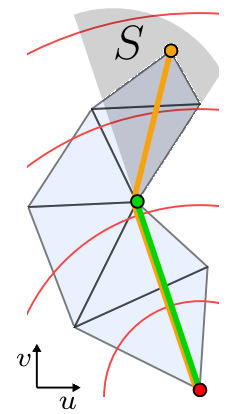
\includegraphics[height=1.5in]{./img/singularity-separation.png}
\end{figure}
}{0.6}{
\begin{block}{}
\begin{eqnarray}
(\Delta u, \Delta v)^T = (u_i,v_i)^T-\eta (u_j,v_j)^T\\
\{sgn(\Delta u)|M\}\cdot \Delta u \geq 1\\
or \{sgn(\Delta v)|M\}\cdot \Delta v \geq 1
\end{eqnarray}
\end{block}
Q: Does this operation guarantee a feasible domain?\\
A: A global scale guarantees it.
}
\end{frame}


\section{Results}
\begin{frame}{Importance of Decimation and Singularity Separation}
\begin{figure}
\centering
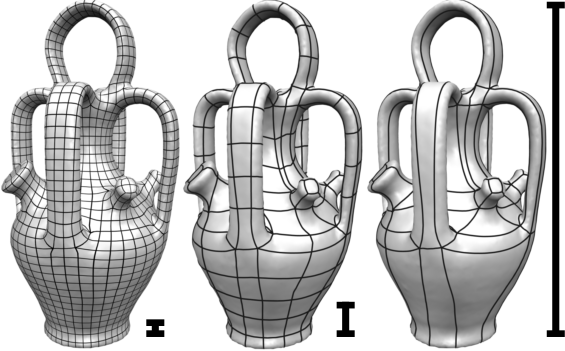
\includegraphics[height=1.2in]{./img/result0.png}
\end{figure}
\begin{itemize}
\item dec(Y),sep(N): can not find solution in 8h
\item dec(N),sep(Y): find a low quality result in 20m for pic 1, and can not find a solution in $8h$ for pic 3.
\item dec(Y),sep(Y): find a result in 17s for pic 3.
\end{itemize}
\end{frame}

\begin{frame}{Compared to greedy rounding}
\begin{figure}
\centering
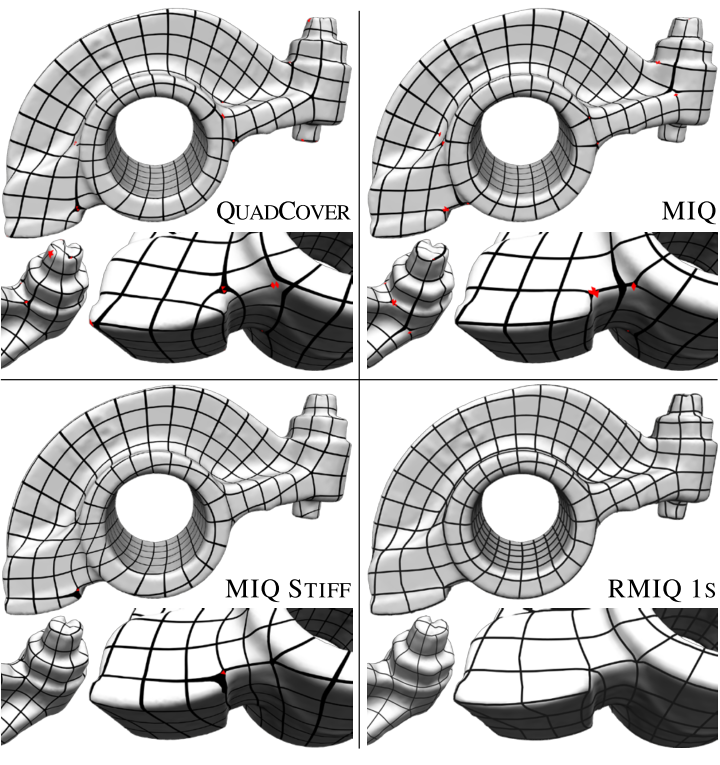
\includegraphics[height=2.8in]{./img/result1.png}
\end{figure}
\end{frame}

\begin{frame}{Reliability}
\begin{figure}
\centering
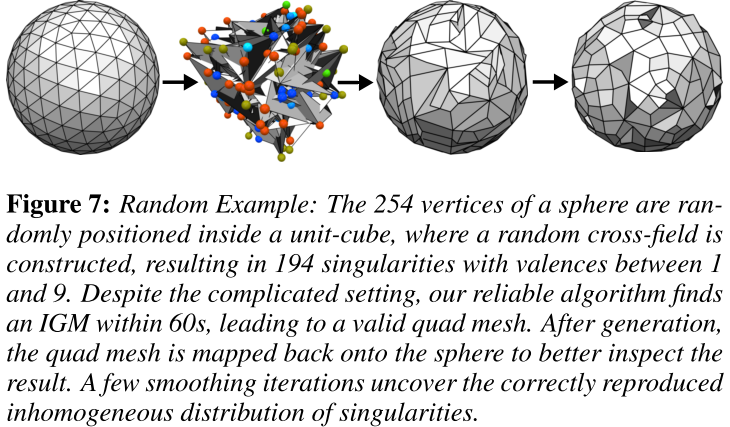
\includegraphics[height=2.5in]{./img/result2.png}
\end{figure}
\end{frame}

\begin{frame}{Complex Models}
\begin{figure}
\centering
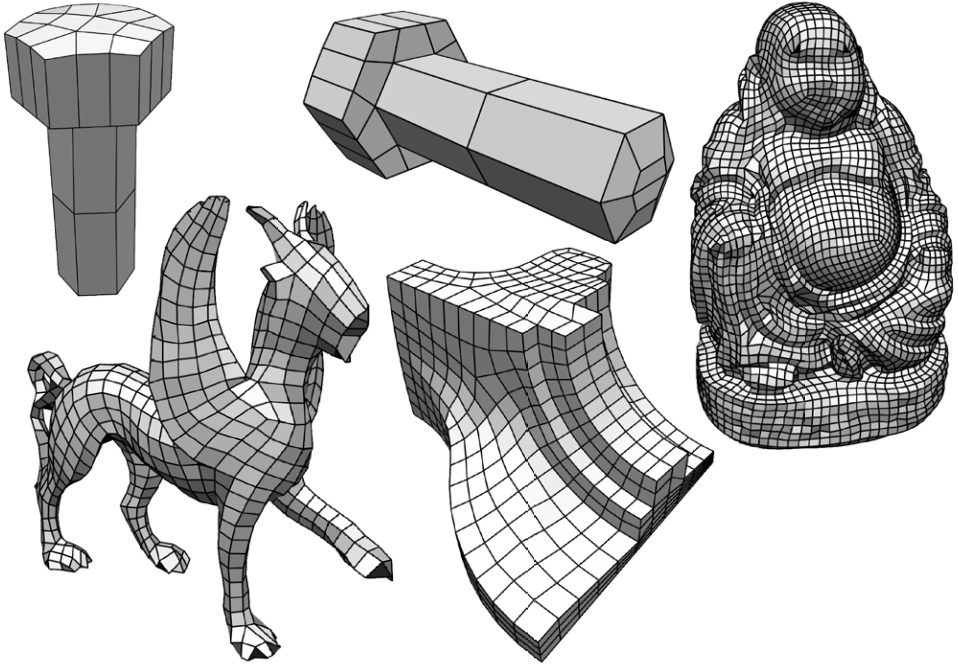
\includegraphics[height=2.5in]{./img/result3.png}
\end{figure}
\end{frame}

\section{Conclusion}
\begin{frame}{Conclusion}
\begin{itemize}
\item Turn functions and contraints to convex form, and get more reliable solution.
\item Engineering style work, but provides interesting insights.
\item Quality of results depends on input size-field and frame field.
\end{itemize}
\end{frame}

\begin{frame}{}
\hspace{1.5in}\huge{Thank you!}
\end{frame}
\end{document}


